\documentclass[11pt]{article}
\usepackage{natbib}
\usepackage{graphicx}
\usepackage{amsmath}
\usepackage{amsfonts}
\usepackage{setspace}
\usepackage{tabulary}
\usepackage{hyperref}
\usepackage[capitalise,noabbrev]{cleveref}
\usepackage[a4paper, total={6in, 8in}]{geometry}
\usepackage{tikz}
\usetikzlibrary{shapes,arrows,positioning}

\tikzset{
    %Define standard arrow tip
    >=stealth',
    %Define style for boxes
    block/.style={
           rectangle,
           draw=black,
           text width=6.5em,
           minimum height=3em,
           text centered},
    % Define arrow style
    arrow/.style={
           ->,
           thick,
           shorten <=2pt,
           shorten >=2pt,
           }
}

\bibliographystyle{plainnat}
\setcitestyle{authoryear,open={(},close={)}}

\newcommand{\pkg}[1]{{\fontseries{b}\selectfont #1}} 


\title{\textbf{How does deindustrialization\\ affect energy intensity?}}
\author{S. Drake Siard}
\date{2020 May 5}
\begin{document}

\maketitle

\begin{abstract}
This project aims to apply a previously developed path model, originally applied to Bangladesh, to analyse the direct and indirect impacts of growth, (de-)industrialization, technological innovation, and trade openness on energy intensity.
The model is first validated by replicating the results in the original paper, and then applied to more recent data in India and the UK.
\end{abstract}

\tableofcontents

\pagebreak

\section{Introduction}
Original paper: \cite{panHowIndustrializationTrade2019}



\section{Data}
 
As in \cite{panHowIndustrializationTrade2019}, the dependent variable is energy intensity (denoted EI). The two independent variables are level of industrialization (ISG)\footnote{
The abbreviation is due to the original paper labelling this as ``Industrial Share of Growth"; however, the measure actually used is industrial share of output, not of output growth. 
Similarly, the variable P\_GDP is a measure of output per capita, not growth.
} and trade openness (TO), and the two intermediary variables are economic output (P\_GDP) and technological innovation (TI).
The precise definitions are described in \cref{tab:data_source} (supplementing Table 2 in \cite{panHowIndustrializationTrade2019}); all data is sampled at an annual frequency.

For the replication phase, in order to most closely match \cite{panHowIndustrializationTrade2019}, it was necessary\footnote{
ISG was revised in the June 2018 vintage, and the ``current" \$US scaler for P\_GDP was rebased in September 2019.
} to use the April 2018 vintage of the data from the WDI Database Archives, \cite{theworldbankWDIDatabaseArchives2018}.
Additional patent data was retrieved directly from the WIPO Statistics Database via the IP Statistics Data Center, \cite{wipoWIPOStatisticsDatabase2020}, and used to fill in gaps in World Bank data where necessary.

For the updated analysis, data was taken directly from the most recent update of the WDI database, \cite{theworldbankWorldDevelopmentIndicators2019}. In addition, an up-to-date alternate energy intensity measure was added from \cite{enerdataGlobalEnergyStatistical2019} and denoted EIb in the dataset.

\begin{table}[htbp]
\centering
\begin{tabulary}{\textwidth}{l l L} 
 Abbr. & Name & Description and units \\ [1ex] 
 \hline 
 EI & Energy intensity & Primary energy use in kg. of oil equivalent per ``current" (2018 or 2019, by dataset) \$US of GDP \\ 
 EIb & Energy intensity & Primary energy use in kg. of oil equivalent per (2015, PPP-adjusted) \$US of GDP \\ 
 ISG & Industrialisation & Total industry (mining, construction, utilities) value added as \% of GDP \\
 TO & Trade openness & Total value of imports and exports (goods and services) as \% of GDP \\ 
 TI & Technological innovation & Total number of patent applications (direct and PCT national phase entries) \\ 
 P\_GDP & Economic output & GDP in ``current" (2018 or 2019, by dataset) \$US, divided by mid-year population \\ 
\end{tabulary}
\caption{Table to test captions and labels}
\label{tab:data_source}
\end{table}

In the original 

\section{Model}

This model is represented in \cref{fig:path_model} (following Figure 3 in \cite{panHowIndustrializationTrade2019})


\begin{figure}[htbp]
\centering
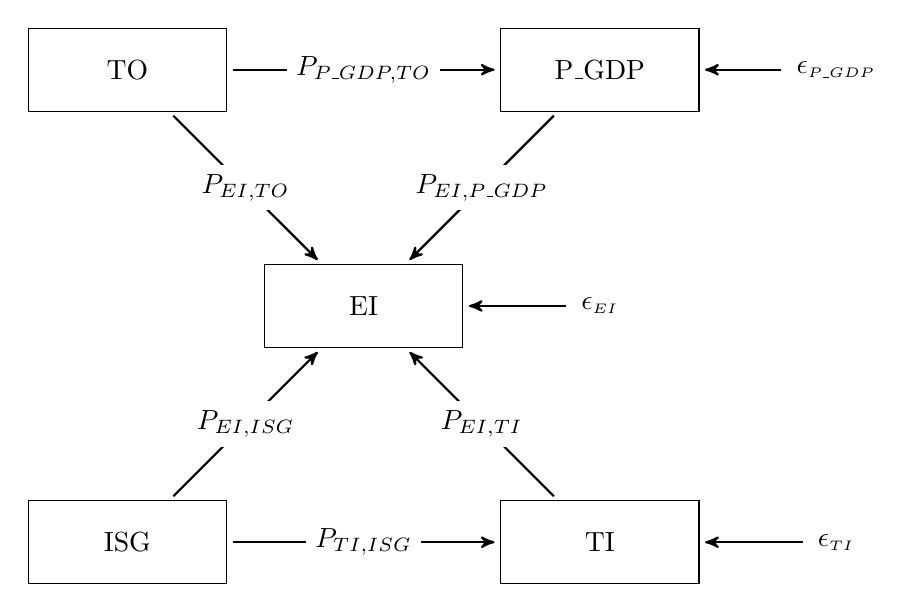
\begin{tikzpicture}[node distance = 3cm, auto]
    \node [block] (EI) {EI};
    \node [above of=EI] (upper dummy) {};    
    \node [below of=EI] (lower dummy) {};    
    \node [block, left of=upper dummy] (TO) {TO};
    \node [block, left of=lower dummy] (ISG) {ISG};
    \node [block, right of=upper dummy] (PGDP) {P\_GDP};
    \node [block, right of=lower dummy] (TI) {TI};
    \node [right of=PGDP] (epsPGDP) {$\epsilon_{\scriptscriptstyle{P\_GDP}}$};
    \node [right of=EI] (epsEI) {$\epsilon_{\scriptscriptstyle{EI}}$};
    \node [right of=TI] (epsTI) {$\epsilon_{\scriptscriptstyle{TI}}$};

	\path[->] (ISG) edge[arrow] node[anchor=center, fill=white] {$P_{EI,ISG}$} (EI);
	\path[->] (ISG) edge[arrow] node[anchor=center, fill=white] {$P_{TI,ISG}$} (TI);
	\path[->] (TO) edge[arrow] node[anchor=center, fill=white] {$P_{EI,TO}$} (EI);
	\path[->] (TO) edge[arrow] node[anchor=center, fill=white] {$P_{P\_GDP,TO}$} (PGDP);
	\path[->] (PGDP) edge[arrow] node[anchor=center, fill=white] {$P_{EI,P\_GDP}$} (EI);
	\path[->] (TI) edge[arrow] node[anchor=center, fill=white] {$P_{EI,TI}$} (EI);
	\path[->] (epsPGDP) edge[arrow] (PGDP);
	\path[->] (epsEI) edge[arrow] (EI);	
	\path[->] (epsTI) edge[arrow] (TI);
\end{tikzpicture}
\caption{Path model for EI, mediated by P\_GDP and TI}
\label{fig:path_model}
\end{figure}

This model was fitted using an R software package for latent variable modeling called \pkg{lavaan}, \cite{rosseelLavaanPackageStructural2012}.



\section{Conclusion}
Maybe.

\clearpage

\appendix
\section{Appendices}

\renewcommand{\refname}{\subsection{References}}.
\bibliography{project}

\subsection{Another appendix}

More lipsum.

\end{document}



\end{document}
